\documentclass{midl}
\jmlrvolume{-- Under Review}
\jmlryear{2027}
\jmlrworkshop{Full Paper -- MIDL 2027 submission}
\editors{Under Review for MIDL 2027}
\usepackage{booktabs}
\title[When does clearing the smoke hurt?]{When Does Clearing the Smoke Hurt? Enhancement, Selection and Abstention for Laparoscopic Segmentation under Controlled Smoke}
\midlauthor{\Name{Nhi-Yen Nguyen-Huynh$^{1}$} \Email{nhinhy23411@st.uel.edu.vn}\\
\addr $^{1}$ Vietnam National University, Ho Chi Minh City -- University of Economics and Law\\
\Name{Nguyen Quoc Khanh Le$^{2}$} \Email{khanhlee@tmu.edu.tw}\\
\addr $^{2}$ Taipei Medical University}
\begin{document}
\maketitle
\begin{abstract}
Smoke from energy devices is usually treated as a preprocessing problem: clear the frame, then segment it. The cleared frame can repair a prediction or overturn a correct one, and mean Dice cannot tell the two apart. We count both events with a paired design in which every enhanced prediction is compared with the unenhanced prediction of the same frozen segmenter on the same frame, using existing AutoLaparo masks, two geometry-preserving smoke simulators (one reserved for final testing), two enhancers (CLAHE and dark-channel-prior dehazing, DCP) and clip-clustered bootstrap intervals. Enhancement harmed far more frames than it helped, including unsmoked ones: DCP lowered uterus Dice from 0.508 to 0.409 on clean frames and harmed 32\% of held-out-smoke frames against 5\% helped. A learned selector between the two predictions improved on always-unenhanced (held-out smoke, DCP: 0.008 [0.002, 0.016]) but not on a foreground-confidence rule (-0.001 [-0.003, 0.002]), and abstention matched confidence ranking. On DeSmoke-LAP, frozen-model confidence barely moves after learned desmoking while predicted masks change, so confidence cannot arbitrate. The results are negative and bounded: synthetic smoke, a frozen model previously exposed to AutoLaparo, no clinical claim. Protocols, manifests and analysis code are released.
\end{abstract}
\begin{keywords}
surgical smoke, image enhancement, segmentation, robustness, selective prediction
\end{keywords}
\section{Introduction}
A surgeon whose view is lost in smoke waits for the evacuator or wipes the lens; a vision pipeline does the software equivalent, clearing the frame and looking again. Desmoking and contrast enhancement are routinely proposed as a front end for recognition~\citep{pan2022desmoke,lu2026seeing}, and the usual argument is that clearer pixels give better predictions.

That argument treats enhancement as extra information. For a fixed segmenter it is also an intervention on the input: it moves colour and texture statistics away from those the model was trained on, and in practice it is applied to frames that contain no smoke at all. Mean Dice does not show how often the enhanced prediction displaces one that was correct, and for a surgeon the two events are not equivalent even when they cancel in a mean.

We study this with a paired design (Figure~\ref{fig:pipe}). Every enhanced prediction is compared with the unenhanced prediction of the same frozen model on the same frame, so each frame is labelled help, harm or unchanged. The comparison pulls three questions apart that accuracy mixes. Does the pair contain a better prediction at all (headroom)? Can a label-free quality score find it (selection)? Can the system decline when neither prediction is reliable (abstention)? Policies are fitted on development smoke and frozen before the held-out family is evaluated.

\begin{figure}[t]
\floatconts{fig:pipe}{\caption{Study overview. (a)~A clean frame with its existing AutoLaparo annotation is corrupted by a seeded smoke simulator (family~A for development, family~B held out), optionally enhanced (none, CLAHE or DCP), and segmented by the frozen joint model. A ridge selector, fitted on development data from label-free features only, picks the raw or enhanced prediction or abstains. (b)~Final-block results: uterus Dice per regime (DCP as enhanced branch), paired Dice change caused by DCP with 95\% CIs, and Dice at 80\% coverage on held-out family~B for the selector versus foreground confidence (fg conf.) and the soft-Dice-style confidence (SDC). Splits: clips 001--170 train, 171--227 validate, 228--300 test.}}
{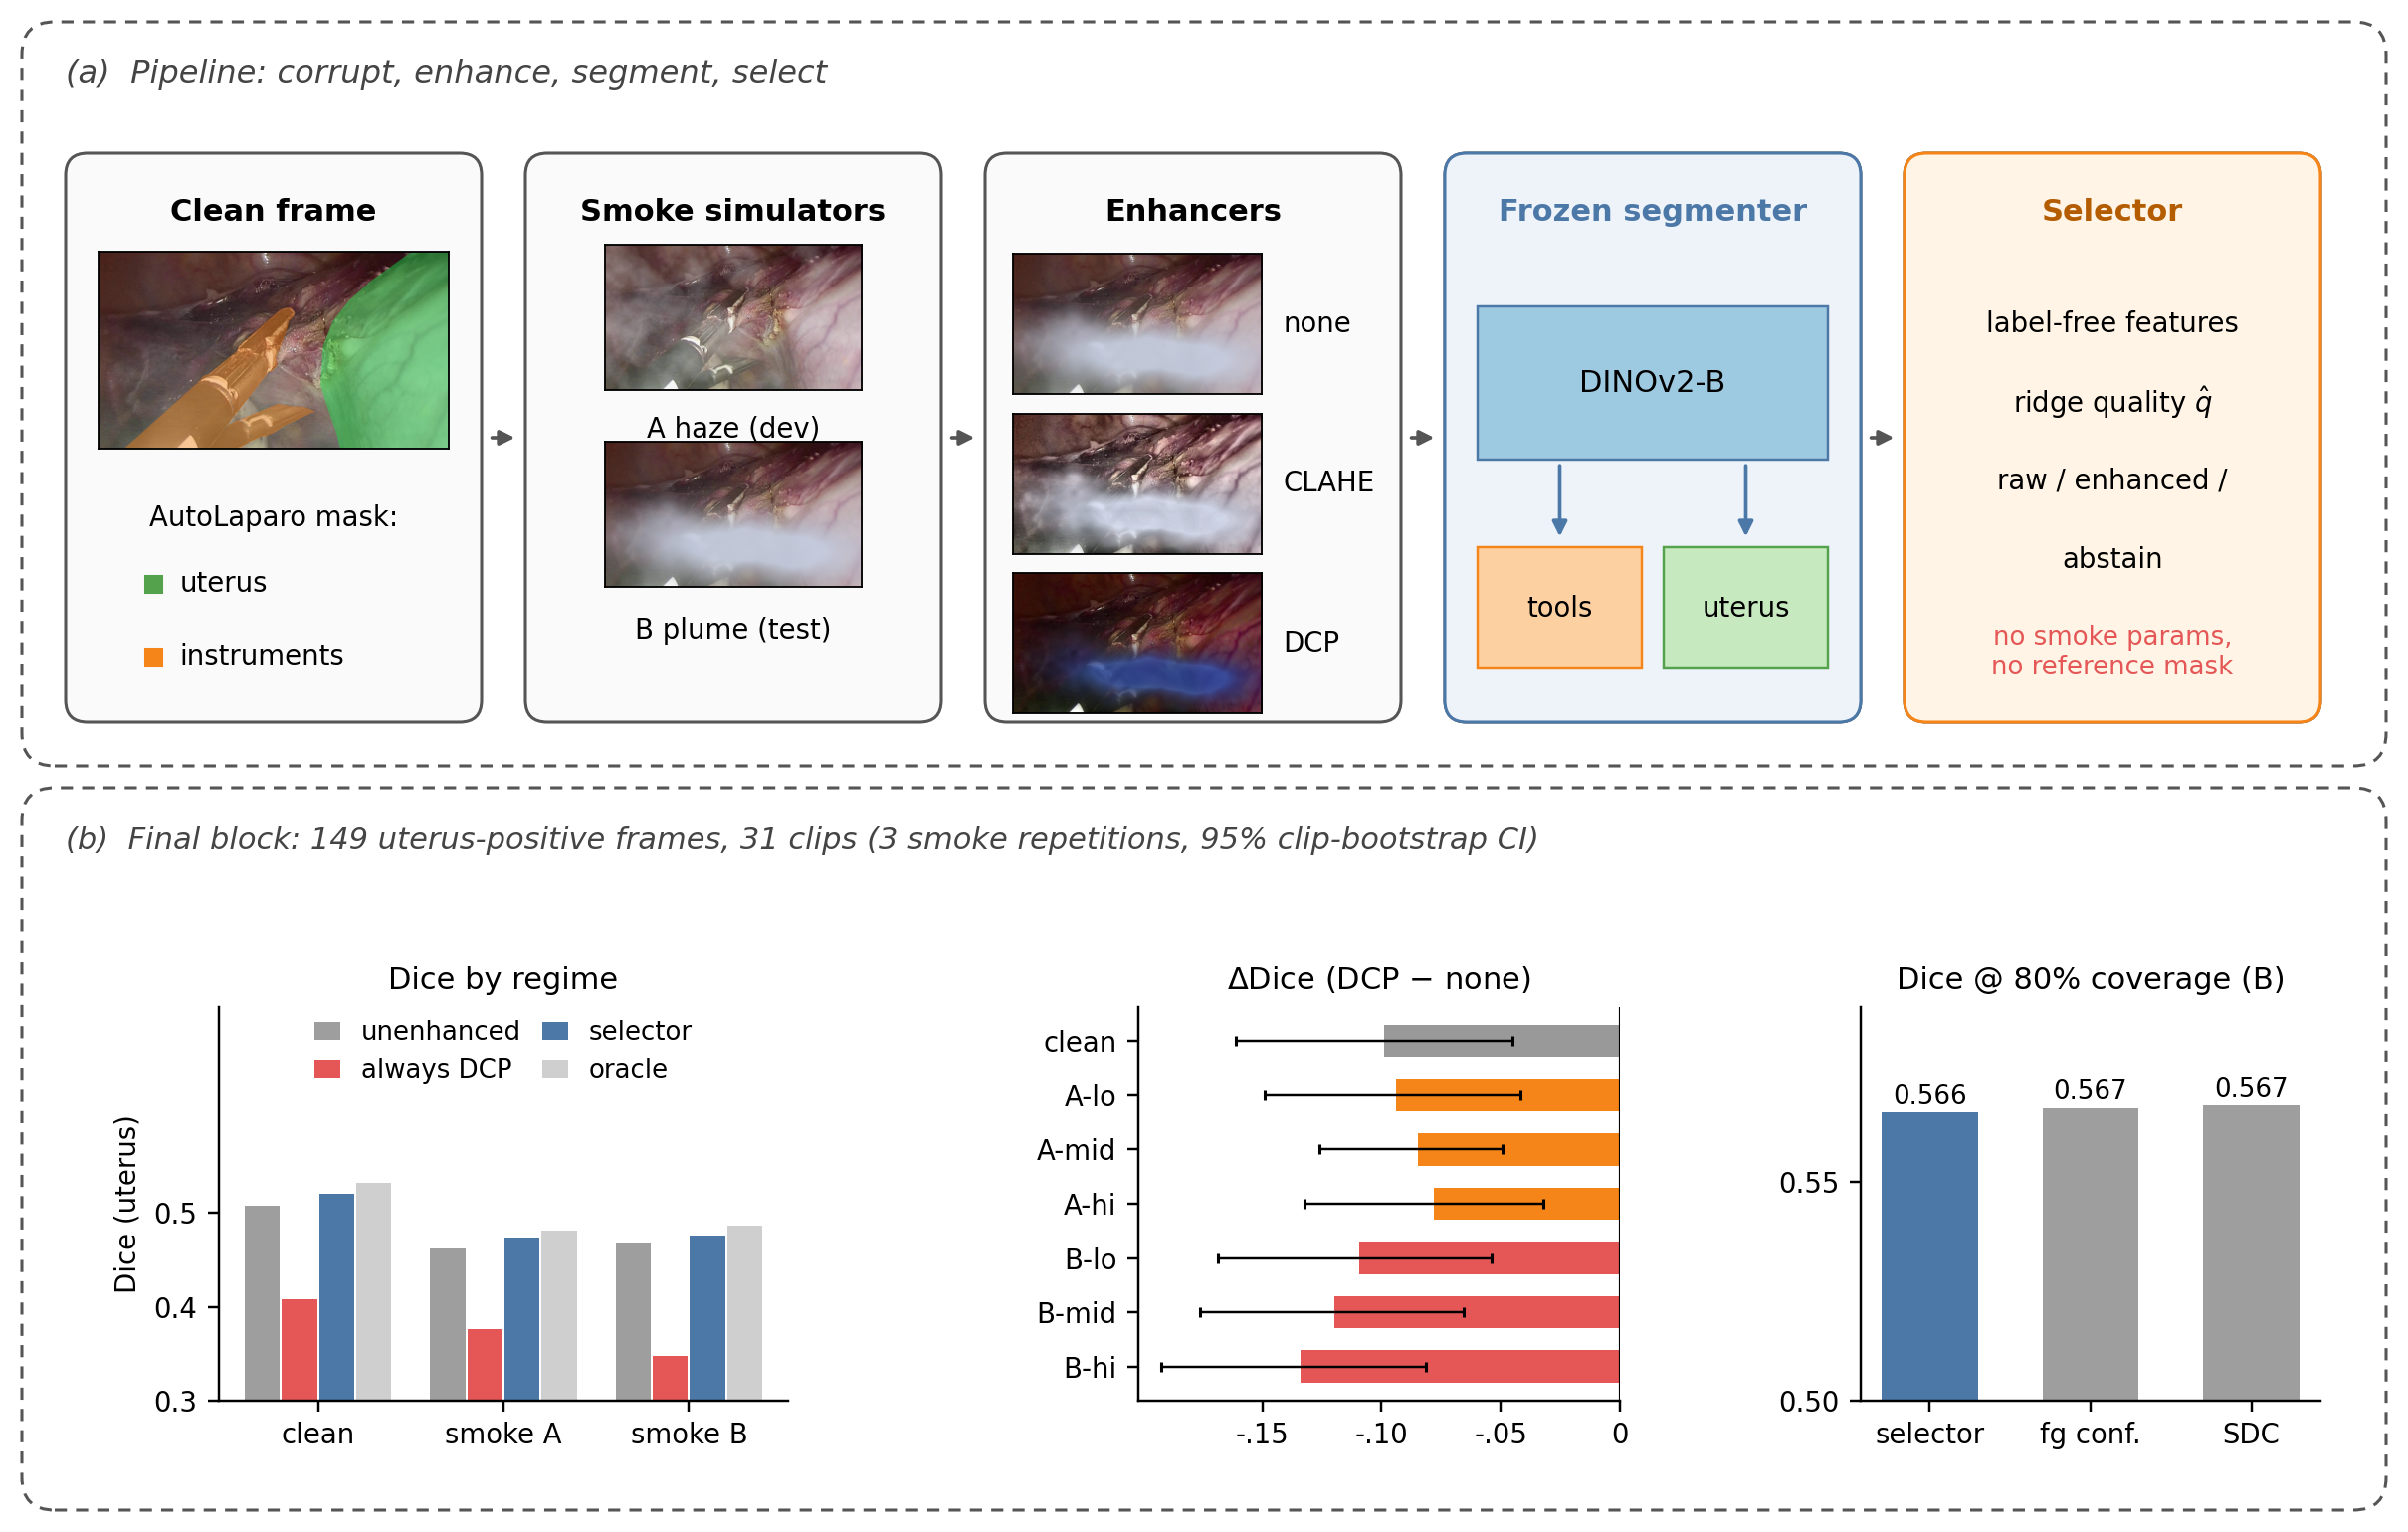
\includegraphics[width=\linewidth]{figs/fig_pipeline.png}}
\end{figure}

The answer to the first question is mostly no. Enhancement harms about a quarter to a third of frames and helps fewer than one in ten, whether or not smoke is present, and the headroom left for a selector is small. A learned selector gains over always-unenhanced but cannot beat a foreground-confidence rule, and abstention behaves identically. We make four contributions. First, a paired protocol and decomposition that reports help, harm, headroom, selection regret and coverage separately, with clip-clustered inference and a held-out smoke family. Second, evidence on two enhancers and two simulators that enhancement does not preserve uterus segmentation on average. Third, a negative result for learned selection and abstention against confidence controls, including a soft-Dice-style confidence. Fourth, descriptive transfer outputs on DeSmoke-LAP with an explicit statement of what they cannot show, together with released protocols and analysis code. A targeted, abstract-level literature check found no study comparing enhanced and unenhanced segmentation branches with abstention under laparoscopic smoke; it was not a systematic review, so we make no strong novelty claim.

\section{Related work}
\textbf{Desmoking and downstream tasks.} Learned desmoking has been proposed for laparoscopy~\citep{pan2022desmoke}, and a recent transformer-based desmoker is evaluated on instrument segmentation and stereo depth, with benefits for the former and inconsistent effects for the latter~\citep{lu2026seeing}. We instead ask whether a fixed, previously trained segmenter benefits at all, including on frames without smoke. \textbf{Robustness and enhancement.} Common-corruption benchmarks~\citep{hendrycks2019corruptions} motivate testing a fixed model under controlled degradations. Enhancers optimised for recognition rather than appearance have been proposed~\citep{son2020urie}, and dehazing has been shown to degrade object detection on clear images, which motivates applying preprocessing selectively~\citep{kumar2025fog}; our segmentation results point in the same direction. 
\textbf{Selective prediction.} Risk--coverage evaluation goes back to~\citet{geifman2017selective}; for segmentation, image-level confidence designed around Dice (Soft Dice Confidence) is a strong estimator~\citep{borges2024sdc}. We include a soft-Dice-style confidence of this kind as an additional control, implemented as an expected-Dice approximation rather than the authors' exact estimator.

\section{Setup and definitions}
For one frame let $D_0$ be the Dice of the unenhanced prediction and $D_e$ that of the prediction after enhancer $e$, and let $G_e=D_e-D_0$. With a margin of $0.05$ fixed before final evaluation we call $G_e>0.05$ \emph{help} and $G_e<-0.05$ \emph{harm}. For a policy $\pi$ that chooses between the two branches let $D_\pi$ be the Dice of its choice and $D^{*}=\max(D_0,D_e)$ the reference-aware oracle, which cannot be deployed. \emph{Headroom} is $\mathrm{HD}=\mathbb{E}[D^{*}-D_0]$, \emph{selection regret} is $\mathrm{RD}(\pi)=\mathbb{E}[D^{*}-D_\pi]$, and \emph{coverage} is the fraction of frames a policy does not abstain on.

\begin{lemma}[Gain bookkeeping]
For any policy $\pi$, $\ \mathbb{E}[D_\pi-D_0]=\mathrm{HD}-\mathrm{RD}(\pi)$.
\end{lemma}
\noindent This is an identity, not a new result: $D_\pi-D_0=(D^{*}-D_0)-(D^{*}-D_\pi)$. Its use is to place a loss: either the enhancer offers little headroom (HD small) or selection wastes what is there (RD large). Table~\ref{tab:hh} reports all three terms.

\textbf{Selector and abstention.} A ridge model predicts the Dice of each branch from label-free features $z$ (confidence, entropy, area, soft-Dice-style confidence, branch disagreement). It picks the branch with the higher predicted Dice $\hat q$, and it abstains when the chosen $\hat q$ falls below a threshold $\tau$ fixed on development data. A selector can only add value beyond a confidence rule if $\hat q$ ranks frames better than confidence does, which is what the risk--coverage comparison tests.

\section{Data, exposure and protocol}
\textbf{AutoLaparo Task 3}~\citep{wang2022autolaparo} provides 1800 frames from 300 clips (six frames per clip) with uterus and instrument masks; 1057 frames have a uterus label. A missing uterus label is not treated as evidence of absence, so the uterus endpoint uses only the 1057 positive frames and instruments are reported as a secondary task on all frames. Instrument parts are merged into one foreground class. Image--mask alignment, label ranges and duplicates were checked automatically (no missing masks, no size mismatches, no duplicate hashes).

\textbf{Prior exposure.} The recognition model is our previously developed joint model (DINOv2-Base~\citep{oquab2024dinov2}, instrument and anatomy heads, frozen checkpoint with recorded SHA-256, no retraining here). All AutoLaparo frames were used as an external test set in that earlier work, and an earlier abandoned fine-tuning experiment on AutoLaparo has unresolved membership. \emph{These data are therefore not independent external validation}; this study measures robustness and selection, not generalisation.

\textbf{Splits.} Procedure identifiers are unavailable. Clip index is used as a proxy; clips 001--170, 171--227 and 228--300 form selector-development, development-validation and final-test blocks, following the contiguous official partition, which likely separates source videos (an assumption that we could not verify). All variants of a frame stay in one block. The final block contains 149 uterus-positive frames from 31 clips. Smoke realisations are not counted as independent samples.

\section{Study design}

\textbf{Smoke simulators} (geometry preserving; masks unchanged). Family~A (development): multi-octave fractal haze blended with a grey-white airlight, three severities (maximum opacity 0.25/0.50/0.75). Family~B (held out, used only for final testing): one to two localised turbulent plumes, bluish or brownish tint, scatter blur and contrast loss, three severities (0.35/0.60/0.85). Severity is defined by simulator parameters, not clinical grading; seeds derive from image, family and severity. Original frames serve as the control.

\textbf{Enhancers.} CLAHE~\citep{zuiderveld1994clahe} on luminance (conventional contrast control) and single-image dark-channel-prior (DCP) dehazing~\citep{he2011dcp} with a guided-filter transmission. The released DeSmoke-LAP weights were not available to us; a learned desmoker is used only on DeSmoke-LAP's released output clips (Section~\ref{sec:ds}). All frames are evaluated at $960{\times}540$ after downscaling.

\textbf{Branches and selector.} Each input yields an unenhanced and an enhanced prediction from the same frozen model. A ridge-regularised quality estimator predicts the Dice of each branch from observable quantities only: mean foreground confidence, mean foreground entropy, predicted area, whole-image mean confidence, branch disagreement (one minus Dice between branches) and a missing-foreground flag. Simulator parameters and reference masks are never inputs. A soft-Dice-style expected-Dice confidence is among the features. The selector picks the branch with higher predicted quality; its abstention score is the predicted quality of the chosen branch. It is fitted on original and family-A frames of the development blocks only; the penalty is chosen on the development-validation block, then refit on all development data and frozen.

\textbf{Controls.} Always unenhanced; always enhanced; confidence only (higher foreground confidence); confidence only on whole-image mean confidence; a disagreement rule (enhanced only if branches agree, threshold tuned on development data); and a reference-aware oracle that serves only as an upper bound. The \emph{strongest simple control} is chosen on development data (here: Confidence only (soft-Dice-style)).

\textbf{Statistics.} Dice is averaged over variants within a frame, frames within a clip, and compared with a clustered bootstrap (4000 resamples of clips). Primary contrast: selector minus the strongest simple control, no abstention, on held-out family~B. Planned contrasts are Holm-adjusted. Secondary: Dice at 80\% coverage ranked by each frozen score, area under the risk--coverage curve (AURC), and deployment thresholds fixed on development data with achieved coverage. Enhancement outcomes: paired Dice change and the share of frames with a drop larger than 0.05 (fixed before final evaluation).

\section{Results}
\subsection{Enhancement lowers uterus Dice, with or without smoke}
Smoke reduces uterus Dice modestly (clip-averaged unenhanced Dice 0.508 on original frames, 0.462 for family~A, 0.469 for family~B; \figureref{fig:deg}). Enhancement did not recover it on average (\tableref{tab:enh}). DCP lowered Dice in every condition, including on original frames (0.409 vs 0.508), with 23--32\% of frames dropping by more than 0.05. Counted per frame (\tableref{tab:hh}), DCP harmed 30\% of clean frames, 25\% under family~A and 32\% under held-out family~B, and helped only 7\%, 6\% and 5\%. CLAHE was gentler (original 0.479) with intervals that include zero for most conditions, but still harmful on average under family~B. Instrument Dice (secondary, \tableref{tab:ins} in the appendix) changes by at most 0.02 and is improved by DCP only under family~A (high and mid severity).

\begin{figure}[!htbp]
\floatconts{fig:deg}{\caption{Uterus Dice versus severity (final block): unenhanced, DCP-enhanced and selector output.}}
{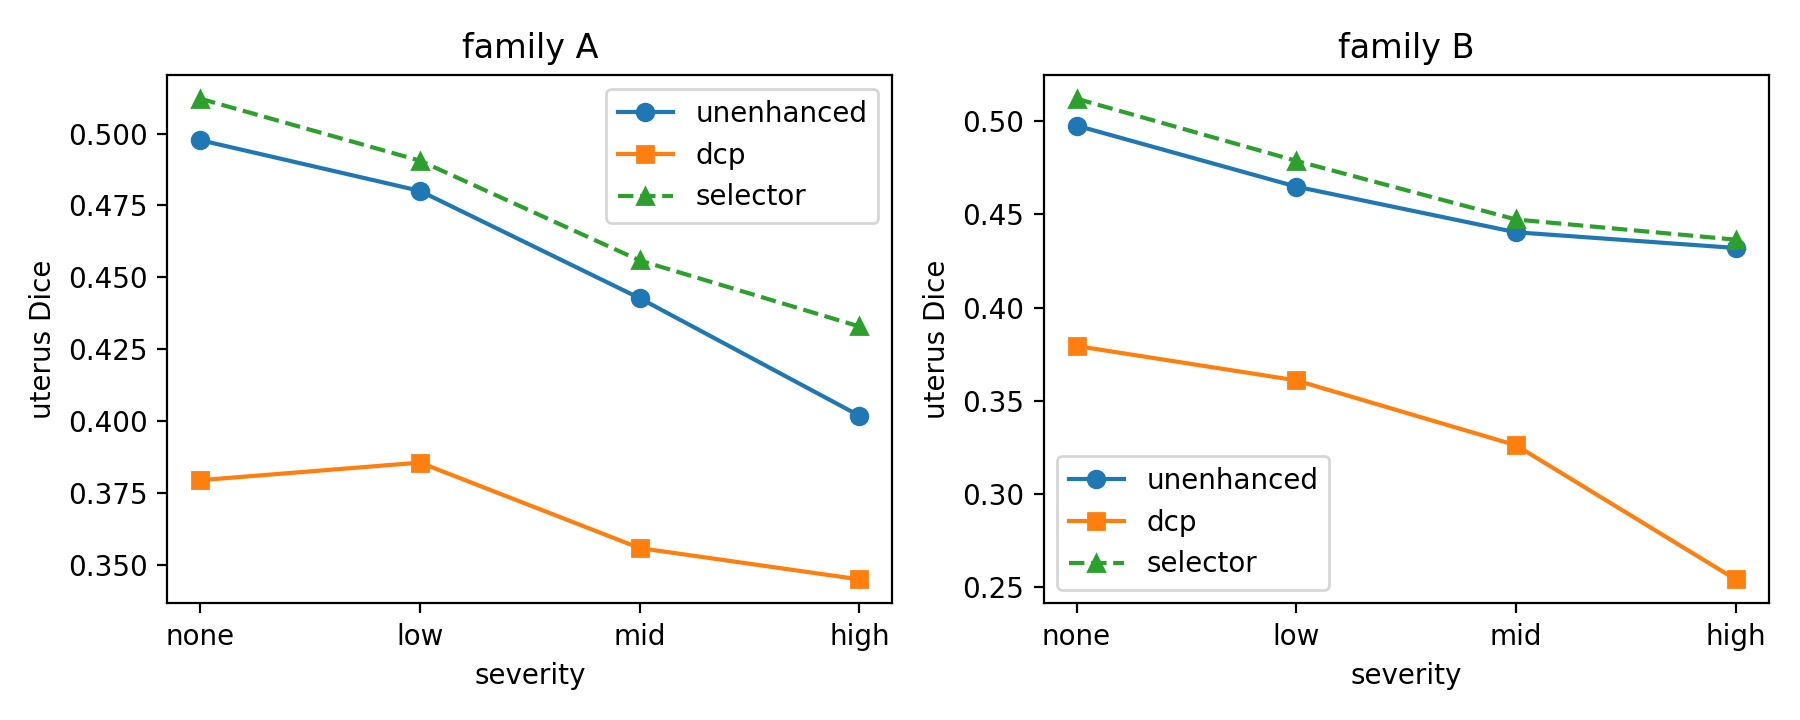
\includegraphics[width=\linewidth]{figs/fig_degradation_recovery.png}}
\end{figure}
\begin{table}[!htbp]
\floatconts{tab:enh}{\caption{Enhancement effect on uterus segmentation, final block (DCP). Dice pooled over frames; $\Delta$ is the clip-averaged paired change [95\% CI]; last column is the share of frames with a drop above 0.05. CLAHE: see Appendix~\ref{app:supp}.}}
{\scriptsize\begin{tabular}{llcccc}\toprule Family & Sev. & Unenh. & Enh. & $\Delta$ & Drop$>$0.05\\\midrule
A & high & 0.413 & 0.335 & -0.078 [-0.132, -0.032] & 23\% \\
A & low & 0.484 & 0.373 & -0.094 [-0.149, -0.042] & 29\% \\
A & mid & 0.444 & 0.355 & -0.085 [-0.126, -0.049] & 24\% \\
B & high & 0.422 & 0.277 & -0.134 [-0.192, -0.081] & 32\% \\
B & low & 0.474 & 0.353 & -0.110 [-0.169, -0.054] & 31\% \\
B & mid & 0.438 & 0.312 & -0.120 [-0.176, -0.066] & 32\% \\
original & none & 0.498 & 0.379 & -0.099 [-0.161, -0.045] & 30\% \\
\bottomrule\end{tabular}}
\end{table}

\begin{table}[!htbp]
\floatconts{tab:hh}{\caption{Help, harm, headroom and regret on the final block (margin 0.05). Help/Harm: share of paired frames with $G_e>0.05$ / $<-0.05$ (pooled over repetitions). $\Delta$ is the mean change of always-enhanced; HD $=\mathbb{E}[D^{*}-D_0]$; Sel. is the selector's gain over unenhanced; RD $=\mathbb{E}[D^{*}-D_\pi]$ for the selector. By the lemma, Sel.\ $=$ HD $-$ RD.}}
{\scriptsize\begin{tabular}{llccccccc}\toprule Enh. & Regime & Help & Harm & $\Delta$ & HD & Sel. & RD\\\midrule
DCP & original & 7.4\% & 29.5\% & -0.099 & 0.025 & +0.013 & 0.011 \\
DCP & A & 5.7\% & 25.4\% & -0.086 & 0.019 & +0.012 & 0.008 \\
DCP & B & 5.1\% & 31.7\% & -0.121 & 0.018 & +0.008 & 0.010 \\
\midrule
CLAHE & original & 7.4\% & 22.1\% & -0.029 & 0.059 & +0.050 & 0.009 \\
CLAHE & A & 9.6\% & 16.9\% & -0.015 & 0.044 & +0.034 & 0.010 \\
CLAHE & B & 8.1\% & 23.9\% & -0.053 & 0.039 & +0.029 & 0.010 \\
\bottomrule\end{tabular}}
\end{table}
\subsection{A learned selector does not beat a confidence rule}
\tableref{tab:main} gives all-case performance. Against always-unenhanced, the selector gained 0.012 for family~A (DCP) and 0.008 [0.002, 0.016] on held-out family~B (DCP; Holm-adjusted $p=0.012$); with CLAHE the held-out gain was 0.029 [0.001, 0.066] and not significant after correction. Against the strongest simple control, which is the foreground-confidence rule, the primary contrast was -0.001 [-0.003, 0.002] ($p_{\mathrm{Holm}}=1.000$; CLAHE: 0.002 [-0.000, 0.004]). \emph{The selector therefore shows no measurable benefit beyond confidence-only selection}, whether the confidence is the foreground mean or the soft-Dice-style expected-Dice score (point differences below 0.002 Dice, intervals within $\pm0.006$). The oracle leaves little headroom over always-unenhanced for DCP (0.487 vs 0.469), which bounds any selector. The strongest simple control was Confidence only (soft-Dice-style) for DCP and Confidence only (foreground) for CLAHE. The selector chose the enhanced branch for 56\% of held-out family-B frames. Whole-image mean confidence is a poor selection signal (\tableref{tab:main}), because background pixels dominate it; the foreground variant is the fair control.

\begin{table}[!htbp]
\floatconts{tab:main}{\caption{Uterus Dice (clip-averaged mean [95\% CI]) on the final block, DCP as enhanced branch. Original = unsmoked frames; A = development smoke family; B = held-out family.}}
{\scriptsize\begin{tabular}{lccc}\toprule Policy & Original & Family A & Family B (held out)\\\midrule
Always unenhanced & 0.508 [0.377, 0.637] & 0.462 [0.334, 0.587] & 0.469 [0.345, 0.595] \\
Always enhanced & 0.409 [0.279, 0.547] & 0.376 [0.249, 0.504] & 0.348 [0.224, 0.471] \\
Confidence only (foreground) & 0.519 [0.385, 0.643] & 0.473 [0.348, 0.596] & 0.477 [0.351, 0.595] \\
Confidence only (whole image) & 0.433 [0.306, 0.566] & 0.403 [0.272, 0.534] & 0.372 [0.244, 0.501] \\
Disagreement rule & 0.507 [0.379, 0.633] & 0.462 [0.332, 0.593] & 0.469 [0.339, 0.595] \\
Confidence only (soft-Dice-style) & 0.520 [0.390, 0.647] & 0.473 [0.343, 0.602] & 0.477 [0.351, 0.602] \\
Learned selector (ours) & 0.521 [0.393, 0.647] & 0.474 [0.350, 0.607] & 0.477 [0.353, 0.602] \\
Oracle (upper bound) & 0.532 [0.401, 0.662] & 0.481 [0.356, 0.607] & 0.487 [0.366, 0.610] \\
\bottomrule\end{tabular}}
\end{table}
\subsection{Abstention adds nothing over confidence ranking}
Risk--coverage curves of the selector and the confidence rule overlap (\figureref{fig:rc}, \tableref{tab:sel}); neither Dice at 80\% coverage nor AURC separates them. With development-fixed thresholds the confidence rule retained 100\% of frames because about 40\% of unenhanced predictions on label-positive frames contain no uterus pixels and receive zero foreground confidence, so the 20th-percentile threshold is degenerate rather than evidence of good calibration. The 80\% coverage setting is a research choice, not a safety standard.

\begin{figure}[!htbp]
\floatconts{fig:rc}{\caption{Risk--coverage curves of the selector quality score and foreground confidence (DCP). Curves overlap.}}
{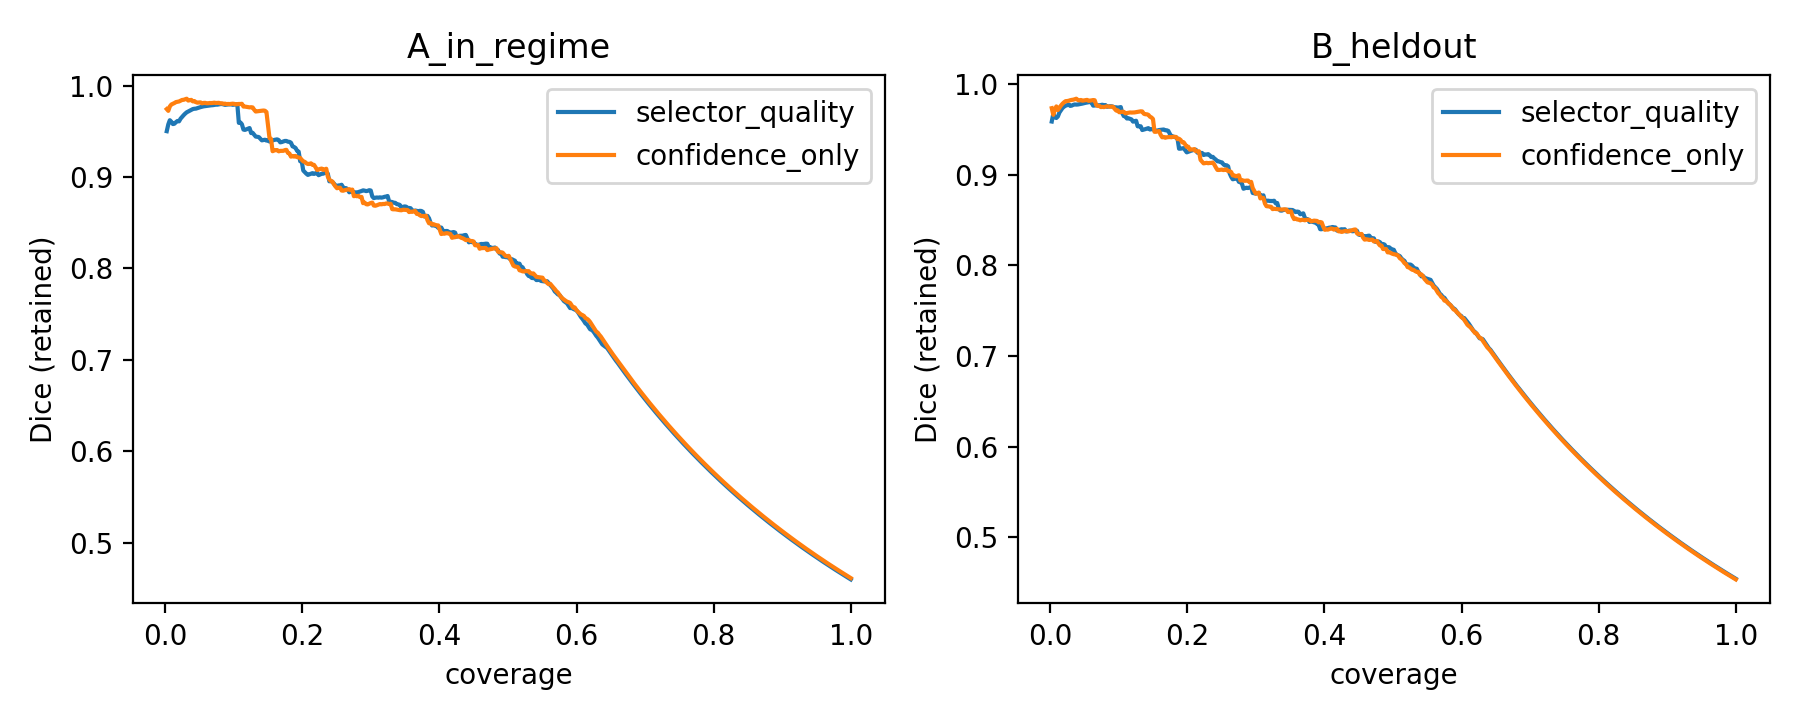
\includegraphics[width=\linewidth]{figs/fig_risk_coverage.png}}
\end{figure}

\subsection{Variability across realisations and cost}
\textbf{Smoke realisations.} Each variant was generated three times with different seeds; results average the realisations within a frame and never count them as independent. Across realisations, held-out family-B unenhanced Dice ranged 0.454--0.478 and DCP-enhanced 0.337--0.356 (family A: 0.455--0.467 and 0.371--0.384), so simulator randomness is small relative to the enhancement effect.

\textbf{Compute.} On one A10 GPU (batch 1, $1920{\times}1080$ JPEG input) the two-branch pipeline took about 130\,ms per frame (median: decoding and resizing 27\,ms, unenhanced branch 10\,ms, CPU DCP 82\,ms, enhanced branch 11\,ms); selector scoring was not timed separately. This is a research measurement, not evidence for real-time surgical use.

\subsection{Real smoke: DeSmoke-LAP outputs are descriptive only}\label{sec:ds} DeSmoke-LAP~\citep{pan2022desmoke} has no organ masks, so no accuracy is reported. On its 500 released test-clip frames, the learned desmoker changed mean uterus-branch confidence from 0.979 to 0.979 and predicted-uterus presence from 30\% to 26\%, while the mean mask disagreement between input and output was 0.191; variation across the ten procedures was large (disagreement 0.032--0.403). Confidence is thus nearly unchanged while masks differ, so confidence alone cannot say whether the changes are corrections or errors. The AutoLaparo-fitted policy picked the enhanced branch for 85\% of these frames and abstained for 45\%, showing that its branch choice and threshold do not transfer across sources; these are not accuracy statements and no claim of confidently wrong anatomy is made.

\begin{table}[!htbp]
\floatconts{tab:ds}{\caption{DeSmoke-LAP descriptive outputs of the frozen pipeline (no reference masks; not accuracy). Pairs show unenhanced / enhanced. Selector and abstention use the AutoLaparo-fitted policy with a development-fixed threshold.}}
{\tiny\begin{tabular}{llrcccrr}\toprule Source & Enhancer & $n$ & Mean conf. & Uterus present & Disagr. & Picks enh. & Abstain\\\midrule
Test clips (input) & CLAHE & 500 & 0.979 / 0.978 & 30\% / 28\% & 0.214 & 83\% & 53\% \\
Test clips (input) & DCP & 500 & 0.979 / 0.982 & 30\% / 15\% & 0.204 & 73\% & 36\% \\
Test clips (input) & DeSmoke-LAP output & 500 & 0.979 / 0.979 & 30\% / 26\% & 0.191 & 85\% & 45\% \\
Clear frames & CLAHE & 600 & 0.979 / 0.977 & 24\% / 26\% & 0.196 & 86\% & 57\% \\
Clear frames & DCP & 600 & 0.979 / 0.981 & 24\% / 16\% & 0.148 & 82\% & 50\% \\
Hazy frames & CLAHE & 600 & 0.975 / 0.975 & 36\% / 34\% & 0.208 & 80\% & 49\% \\
Hazy frames & DCP & 600 & 0.975 / 0.979 & 36\% / 23\% & 0.235 & 70\% & 40\% \\
\bottomrule\end{tabular}}
\end{table}

\section{Discussion and limitations}
What clearing the smoke is worth belongs to the model and its training distribution, not to enhancement as such. With this frozen segmenter both enhancers cost Dice on average, even where there is no smoke to remove, so the enhancer changes the input in a way the model does not absorb. Three practical lessons follow. Report help and harm separately: a small mean loss hides that roughly a third of held-out-smoke frames get worse. Compare any learned selector with always-unenhanced \emph{and} with a confidence rule before claiming learned selection, because here the gap to the confidence control is about 0.00 Dice. And do not treat confidence as a check on enhancement: on DeSmoke-LAP confidence stays near its ceiling while masks differ substantially.

\textbf{Limitations.} Results concern two simulators, three realisations each, and downscaled frames; real smoke differs. The frozen model reaches only moderate uterus Dice on these frames (0.508), was previously exposed to AutoLaparo, and enhancement operates on frames the model was never adapted to; a model trained on enhanced data could behave differently. Clip index is a proxy for procedure and independence of the blocks is assumed. The two enhancers are simple; the strongest learned desmoker was not run on AutoLaparo. The uterus endpoint excludes 743 frames without labels. The analysis was fixed after a first pass in which the whole-image confidence control was found to be a weak baseline; we replaced it by the foreground control and report both; the soft-Dice-style control and the three-fold repetition of smoke realisations were added afterwards in response to the literature check. These post hoc additions did not change the primary conclusion, but the primary-contrast control is defined by the development-data rule stated above. Nothing here establishes accuracy under real smoke, recognition of hidden anatomy, clinical benefit, or real-time suitability (timing above is a research measurement on one GPU). Following the pre-specified decision point, we narrow the claim: under these conditions we found no evidence that a learned selector improves on a confidence rule, and we do not present this as a method contribution.

\section{Conclusion}
Enhancement before segmentation is not safe by default: it lowered uterus Dice on average even on unsmoked frames. Choosing between branches helps relative to always-unenhanced, but a foreground-confidence rule matches the learned selector, and abstention adds nothing measurable. Future work should evaluate on independent annotated cohorts with verified procedure identifiers, add real-smoke references, and test enhancers trained jointly with the segmenter.

\section*{Ethics Statement}
This study uses two released research datasets (AutoLaparo and DeSmoke-LAP) under their non-commercial licences, creates no new patient data, and offers no clinical recommendation. Smoke is simulated, so no conclusion about real surgical smoke or patient outcomes should be drawn.

\section*{Data and Code Availability}
Code, protocols, manifests with content hashes, per-case results and analysis outputs: \url{https://github.com/nhynhi23411/MIDL2027_Smoke_Enhancement_Selection}. AutoLaparo and DeSmoke-LAP images and the frozen checkpoint are not redistributed; image identifiers, hashes and seeds allow every perturbed frame to be rebuilt from the original sources.

\section*{Use of AI tools}
An AI assistant (Claude, Anthropic) was used for writing and running analysis scripts, language edits, consistency checks of the text and reference verification, under the authors' direction. The authors designed the study, checked all results, and take full responsibility for the paper.

\midlacknowledgments{This research was funded by the University of Economics and Law, Ho Chi Minh City, Vietnam, and Vietnam National University, Ho Chi Minh City, Vietnam. The datasets AutoLaparo and DeSmoke-LAP are used under their respective licences.}
\bibliography{refs}
\appendix
\section{Supplementary results}
\label{app:supp}
Tables~\ref{tab:con} and~\ref{tab:sel} give all planned contrasts and the selective-prediction summary for DCP. Tables~\ref{tab:mainc} and~\ref{tab:enhc} repeat the main comparison and the enhancement effect with CLAHE as the enhanced branch; Table~\ref{tab:ins} gives the secondary instrument endpoint.
\begin{table}[htbp]
\floatconts{tab:mainc}{\caption{As Table~\ref{tab:main} with CLAHE as the enhanced branch.}}
{\scriptsize\begin{tabular}{lccc}\toprule Policy & Original & Family A & Family B (held out)\\\midrule
Always unenhanced & 0.508 [0.377, 0.637] & 0.462 [0.334, 0.587] & 0.469 [0.345, 0.595] \\
Always enhanced & 0.479 [0.343, 0.616] & 0.447 [0.326, 0.572] & 0.416 [0.288, 0.541] \\
Confidence only (foreground) & 0.551 [0.419, 0.673] & 0.494 [0.372, 0.614] & 0.496 [0.371, 0.613] \\
Confidence only (whole image) & 0.479 [0.346, 0.611] & 0.436 [0.310, 0.561] & 0.418 [0.293, 0.545] \\
Disagreement rule & 0.508 [0.379, 0.633] & 0.462 [0.332, 0.593] & 0.469 [0.339, 0.595] \\
Confidence only (soft-Dice-style) & 0.559 [0.435, 0.675] & 0.497 [0.374, 0.621] & 0.499 [0.372, 0.618] \\
Learned selector (ours) & 0.558 [0.435, 0.680] & 0.496 [0.374, 0.624] & 0.497 [0.375, 0.621] \\
Oracle (upper bound) & 0.567 [0.439, 0.690] & 0.506 [0.385, 0.625] & 0.508 [0.387, 0.631] \\
\bottomrule\end{tabular}}
\end{table}
\begin{table}[htbp]
\floatconts{tab:enhc}{\caption{As Table~\ref{tab:enh} with CLAHE.}}
{\scriptsize\begin{tabular}{llcccc}\toprule Family & Sev. & Unenh. & Enh. & $\Delta$ & Drop$>$0.05\\\midrule
A & high & 0.413 & 0.398 & -0.010 [-0.046, 0.029] & 15\% \\
A & low & 0.484 & 0.425 & -0.027 [-0.089, 0.042] & 20\% \\
A & mid & 0.444 & 0.411 & -0.007 [-0.056, 0.048] & 16\% \\
B & high & 0.422 & 0.345 & -0.064 [-0.112, -0.015] & 25\% \\
B & low & 0.474 & 0.401 & -0.043 [-0.107, 0.024] & 22\% \\
B & mid & 0.438 & 0.363 & -0.051 [-0.113, 0.007] & 25\% \\
original & none & 0.498 & 0.427 & -0.029 [-0.111, 0.063] & 22\% \\
\bottomrule\end{tabular}}
\end{table}
\begin{table}[htbp]
\floatconts{tab:ins}{\caption{Instrument union Dice (secondary, all final-block frames) by enhancer.}}
{\scriptsize\begin{tabular}{llccc}\toprule Family & Sev. & Unenh. & CLAHE & DCP\\\midrule
A & high & 0.850 & 0.829 & 0.867 \\
A & low & 0.899 & 0.886 & 0.890 \\
A & mid & 0.881 & 0.866 & 0.885 \\
B & high & 0.849 & 0.828 & 0.835 \\
B & low & 0.897 & 0.892 & 0.888 \\
B & mid & 0.886 & 0.879 & 0.883 \\
orig. & none & 0.903 & 0.896 & 0.898 \\
\bottomrule\end{tabular}}
\end{table}
\begin{table}[htbp]
\floatconts{tab:con}{\caption{Selector minus control, Dice difference [95\% CI] and Holm-adjusted $p$ (all planned contrasts per enhancer). $^\dagger$ primary contrast. Top: DCP; bottom: CLAHE.}}
{\scriptsize\begin{tabular}{llcc}\toprule Family & Control & Difference & $p_{\mathrm{Holm}}$\\\midrule
A & Always unenhanced & 0.012 [0.006, 0.019] & 0.000 \\
A & Confidence only (foreground) & 0.001 [-0.002, 0.003] & 1.000 \\
A & Confidence only (soft-Dice-style) & 0.001 [-0.001, 0.002] & 1.000 \\
A & Disagreement rule & 0.012 [0.006, 0.019] & 0.000 \\
B & Always unenhanced & 0.008 [0.002, 0.016] & 0.012 \\
B & Confidence only (foreground) & -0.000 [-0.003, 0.003] & 1.000 \\
B & Confidence only (soft-Dice-style)$^{\dagger}$ & -0.001 [-0.003, 0.002] & 1.000 \\
B & Disagreement rule & 0.008 [0.002, 0.016] & 0.025 \\
\midrule
A & Always unenhanced & 0.034 [0.005, 0.072] & 0.068 \\
A & Confidence only (foreground) & 0.002 [-0.000, 0.006] & 0.396 \\
A & Confidence only (soft-Dice-style) & -0.001 [-0.002, 0.000] & 0.396 \\
A & Disagreement rule & 0.034 [0.005, 0.074] & 0.068 \\
B & Always unenhanced & 0.029 [0.001, 0.066] & 0.222 \\
B & Confidence only (foreground)$^{\dagger}$ & 0.002 [-0.000, 0.004] & 0.308 \\
B & Confidence only (soft-Dice-style) & -0.001 [-0.006, 0.002] & 0.492 \\
B & Disagreement rule & 0.029 [0.000, 0.065] & 0.225 \\
\bottomrule\end{tabular}}
\end{table}
\begin{table}[htbp]
\floatconts{tab:sel}{\caption{Selective prediction on the final block (DCP). Dice at 80\% coverage and AURC use ranking by each frozen score; the last two columns use the threshold fixed on development data.}}
{\scriptsize\begin{tabular}{llccccc}\toprule Fam. & Score & Dice@80\% & AURC & Cov. & Dice (kept)\\\midrule
A & selector quality & 0.574 & 0.232 & 70\% & 0.655 \\
A & fg confidence & 0.574 & 0.235 & 100\% & 0.460 \\
A & soft-Dice conf. & 0.574 & 0.229 & 100\% & 0.460 \\
B & selector quality & 0.566 & 0.238 & 70\% & 0.649 \\
B & fg confidence & 0.567 & 0.239 & 100\% & 0.454 \\
B & soft-Dice conf. & 0.567 & 0.234 & 100\% & 0.454 \\
\bottomrule\end{tabular}}
\end{table}
\section{Policy definitions}
\begin{table}[htbp]
\floatconts{tab:pol}{\caption{Frozen policies. $\lambda$: ridge penalty chosen on the development-validation block; thr.: disagreement threshold of the disagreement rule; strongest control: chosen on development data; $\tau_{80}$: abstention threshold giving 80\% coverage on development data; $n_{\mathrm{dev}}$: label-positive development images; picks enh.: share of held-out family-B frames for which the selector picks the enhanced branch.}}
{\scriptsize\begin{tabular}{lcclccc}\toprule Enh. & $\lambda$ & thr. & Strongest control & $\tau_{80}$ & $n_{\mathrm{dev}}$ & Picks enh.\\\midrule
DCP & 1000 & 0.02 & Confidence only (soft-Dice-style) & 0.024 & 908 & 56\% \\
CLAHE & 1000 & 0.00 & Confidence only (foreground) & 0.034 & 908 & 57\% \\
\bottomrule\end{tabular}}
\end{table}
\textbf{Simulators.} Family~A: multi-octave fractal haze (five octaves), grey-white airlight $(0.86,0.86,0.88)$, coverage $0.45/0.60/0.75$ and maximum opacity $0.25/0.50/0.75$ for low/mid/high. Family~B: one or two Gaussian plumes warped by fractal noise, bluish or brownish tint, scatter blur with $\sigma=3+6\alpha_{\max}$ and contrast loss $1-0.5\alpha$, maximum opacity $0.35/0.60/0.85$. \textbf{Features.} Foreground confidence, foreground entropy, predicted area, whole-image confidence, branch disagreement, soft-Dice-style expected-Dice confidence, a missing-foreground flag and a branch indicator; features are standardised on development data. \textbf{Enhancers.} CLAHE clip limit 3.0 on an $8{\times}8$ grid applied to LAB luminance; DCP with a $15{\times}15$ patch, $\omega=0.95$, transmission floor $0.1$ and a guided filter of radius 41.

\section{Reproducibility details}
Frozen checkpoint SHA-256 \texttt{c8c76331\ldots}; code, simulator configuration, split and exposure tables are released at \url{https://github.com/nhynhi23411/MIDL2027_Smoke_Enhancement_Selection}. Smoke seeds are derived deterministically from image name, family, severity and repetition index (three repetitions). Both enhancers and the selector are deterministic given the seeds.
\end{document}
